
\subsection{SD-based optimization strategies}\label{S:SD}

\subsubsection{SD dispersion measure}

Standard deviation, \SD, is a special case, for $p=2$, of central momentum dispersion measure defined
in Eq.~(\ref{cmdm1}), \ie,
\begin{equation}
    \SD = \sqrt{\VAR(r)},
    \label{sd01}
\end{equation}
where $\VAR(r)$ is the variance of the rate of return. For a portfolio, defined by the set of weights $\{w_k\}_{k=1,\cdots,M}$,
Eq.~(\ref{sd01}) can be rewritten as
\begin{equation}
    \SD = \sqrt{w^T\cdot C\cdot w},
    \label{sd02}
\end{equation}
where $C$ is the covariance matrix between the portfolio components.
Although for direct computations either Eq.~(\ref{sd01}) or
Eq.~(\ref{sd0}) is sufficient, it is useful to mention the following alternative expression
\begin{equation}
    \SD = \| U\cdot w \|_2,
    \label{sd0}
\end{equation}
where $\|\cdot\|_2$ is the Euclidian norm and $U$ is a matrix such that $U^T\cdot U = C$. In general, $U$ is not unique.
If $C$ is a positive defined matrix, then $U$ can be given by the
Cholesky factorization. If $C$ is only positive semidefinite,\footnote{$C$ can be semidefinite if one of the portfolio components
is a risk-free asset (with zero volatility), \eg\ a pure cash position. \azapy\ implementation covers these cases too.} then $U$ can be computed as the
square root matrix.\footnote{The square root matrix of $C$ is the unique semidefinite matrix $U$ such that $U\cdot U = C$.}

\BackToContents


\subsubsection{SD optimal portfolio}
This optimization is described by Eqs.~(\ref{gg1}) from Sec~\ref{strategies} point~\ref{OptRisk},
where $\rho$ is given by \SD\ from Eq.\ (\ref{sd0}).
It is the following SOCP problem.

\bigskip
\noindent Minimize over $\{ \{w_k\}_{k=1,\cdots,M}, \eta \}$
\begin{subequations}\label{sd1}
\begin{align}
    & g = \eta, \label{sd1a} \\
    \st & \| U w \|_2 \leq \eta, \label{sd1b} \\
        & \sum_{k=1}^M w_k \mu_k \geq \mu_0, \label{sd1c} \\
        & \sum_{k=1}^K w_k = 1, \label{sd1d} \\
        & \eta \geq 0, \label{sd1f} \\
        & w_k \geq 0, \label{sd1e}
\end{align}
\end{subequations}

\noindent where $\mu$ from Eq.~(\ref{sd1c})
is the targeted portfolio rate of return, while $\mu_k$ for $k=1,\cdots,M$
are the portfolio components expected rate of returns.
Then, we have
\begin{subequations}\label{sd2}
\begin{align}
    \RR &= \sum_{k=1}^M w_k^* \mu_k, \label{sd2a} \\
    \SD &= g^*, \label{sd2b}
\end{align}
\end{subequations}

\noindent where $^*$ denotes the solution of SOCP problem.
In addition to the optimal portfolio weights $\{w_k^*\}_{k=1,\cdots,M}$ and expected
rate of return $\RR$, the
SOCP solution provides information about the portfolio standard deviation \SD.

\bigskip
\noindent Here is an example, using the \azapy\ package, of how to compute the \SD\ optimal portfolio.
The \SD\ time horizon was set to one quarter and the calibration is performed using 3.25 years of
close-adjusted historical prices (default settings).
For more details see the package documentation at \azapydoc.

\lstinputlisting[language=Python]{../PyScripts/SD_RiskOptim.py}

\BackToContents


\subsubsection{Minimum SD portfolio}

Following the results from Sec.~\ref{strategies} point~\ref{MinRisk},
the algorithm to compute the optimal portfolio with minimum \SD\ is given by the SOCP problem from Eqs.~(\ref{sd1}) where
$\mu$ from r.h.s. of Eq.~(\ref{sd1c}) is set to a value equal to the smallest expected rate of
return among the portfolio components, \ie\ $\mu=\min_k\{\mu_k\}$.

\bigskip
\noindent Here is an example, using the \azapy\ package, of how to compute the minimum \SD\ portfolio.
The \SD\ time horizon was set to one quarter and the calibration is performed using 3.25 years of
close-adjusted historical prices (default settings).
For more details see the package documentation at \azapydoc.

\lstinputlisting[language=Python]{../PyScripts/SD_MinRisk.py}

\BackToContents


\subsubsection{SD optimal portfolio for targeted risk value}
This optimization is described by Eqs.~(\ref{gg2}) from Sec.~\ref{strategies} point~\ref{TargetRisk},
where $\rho$ given by \SD\ from Eq.\ (\ref{sd0}).
It is the following SOCP problem.

\bigskip
\noindent Maximize over $\{ w_k \}_{k=1,\cdots, M}$
\begin{subequations}\label{sd3}
\begin{align}
    & g = \sum_{k=1}^M w_k \mu_k, \label{sd3a} \\
    \st & \| U w\|_2 \leq \SD_0, \label{sd3b} \\
        & \sum_{k=1}^M w_k = 1, \label{sd3c} \\
        & w_k \geq 0, \label{sd3d}
\end{align}
\end{subequations}

\noindent where $\SD_0$ from Eq.~(\ref{sd3b}) is the targeted portfolio \SD\ value.
The portfolio expected rate of return is given by the optimal value of the objective
function, \ie,
\begin{equation}
    \RR = g^*, \label{sd4}
\end{equation}

\noindent and the optimal portfolio weights by $\{w^*_k\}_{k=1,\cdots,M}$. The superscript $^*$ denotes the
solution of SOCP problem.


\bigskip
\noindent Here is an example, using the \azapy\ package, of how to compute the optimal portfolio
with the same \SD\ as the equal weighted portfolio.
The \SD\ time horizon was set to one quarter and the calibration is performed using 3.25 years of
close-adjusted historical prices (default settings).
For more details see the package documentation at \azapydoc.

\lstinputlisting[language=Python]{../PyScripts/SD_InvNrisk.py}

\BackToContents


\subsubsection{SD optimal portfolio for fixed risk-aversion factor}
This optimization is described by Eqs.~(\ref{gg3}) from Sec.~\ref{strategies} point~\ref{RiskAverse},
where $\rho$ is given by \SD\ from Eq.\ (\ref{sd0}).
It is the following SOCP problem.

\bigskip
\noindent Maximize over $\{ \{w_k\}_{k=1,\cdots,M}, \eta \}$
\begin{subequations}\label{sd5}
\begin{align}
    & g = \sum_{k=1}^M w_k \mu_k -\lambda \eta, \label{sd5a} \\
    \st & \| U w\|_2 \leq \eta, \label{sd5b} \\
        & \sum_{k=1}^m w_k = 1, \label{sd5c} \\
        & \eta \geq 0, \label{sd5e} \\
        & w_k \geq 0, \label{sd5d}
\end{align}
\end{subequations}

\noindent where $\lambda$ from Eq.~(\ref{sd5a}) is the risk-aversion factor.
Then, we have
\begin{subequations}\label{sd6}
\begin{align}
    \RR &= \sum_{k=1}^M w_k^* \mu_k, \label{sd6a} \\
    \SD &= \eta^*, \label{sd6b}
\end{align}
\end{subequations}

\noindent where $^*$ denotes the solution of SOCP problem.
In addition to the optimal portfolio weights $\{w_k^*\}_{k=1,\cdots,M}$ and expected rate of return $\RR$, the
SOCP solution provides information about the portfolio \SD.

\bigskip
\noindent Here is an example, using the \azapy\ package, of how to compute the optimal portfolio
for a given value of the risk-aversion factor $\lambda$.
The \SD\ time horizon was set to one quarter and the calibration is performed using 3.25 years of
close-adjusted historical prices (default settings).
For more details see the package documentation at \azapydoc.

\lstinputlisting[language=Python]{../PyScripts/SD_Averse.py}

\BackToContents


\subsubsection{Sharpe optimal portfolio - maximization solution}
This optimization targets the maximization of Sharpe ratio. It is based on
Eqs.~(\ref{gg4}) from Sec.~\ref{strategies} point~\ref{MaxSharpe},
where $\rho$ is given by \SD\ from Eq.~(\ref{sd0}).
The optimization can be formulated as an SOCP problem
if Eq.~(\ref{gg4b}) can be expressed as a second order cone constraint.  This can be achieved by
introducing the variable transformations $\bw_k = t w_k$. Then, the SOCP
problem can be written as follows.

\bigskip
\noindent Maximize over $\{ \{\bw_k\}_{k=1,\cdots,M}, t\}$
\begin{subequations}\label{sd7}
\begin{align}
    & g = \sum_{k=1}^M \bw_k \mu_k - \mu_0 t, \label{sd7a} \\
    \st & \| U \bw \|_2 \leq 1, \label{sd7b} \\
        & \sum_{k=1}^M \bw_k - t = 0, \label{sd7c} \\
        & t \geq 0, \label{sd7e} \\
        & \bw_k \geq 0, \label{sd7d}
\end{align}
\end{subequations}

\noindent where $\mu_0$ from Eq.~(\ref{sd7a}) is the risk-free rate accessible to the investor.
Then, we have
\begin{subequations}\label{sd8}
\begin{align}
    w_k &= \frac{\bw_k^*}{t^*}, \label{sd8a} \\
    \RR &= \frac{g^*}{t^*} + \mu_0, \label{sd8c} \\
    \Sharpe &= g^*, \label{sd8b} \\
    \SD &= \frac{1}{t^*}, \label{sd8d}
\end{align}
\end{subequations}

\noindent where $^*$ denotes the solution of SOCP problem.
In addition to the optimal portfolio weights $\{w_k\}_{k=1,\cdots,M}$, expected rate of return $\RR$ and
the Sharpe ratio $\Sharpe$,
the SOCP solution provides information about the portfolio \SD.


\bigskip
\noindent Here is an example, using the \azapy\ package, of how to compute the Sharpe optimal portfolio using the maximization
of Sharpe ratio.
The \SD\ time horizon was set to one quarter and the calibration is performed using 3.25 years of
close-adjusted historical prices (default settings).
For more details see the package documentation at \azapydoc.

\lstinputlisting[language=Python]{../PyScripts/SD_Sharpe.py}

\BackToContents


\subsubsection{Sharpe optimal portfolio - minimization solution}
This optimization targets the minimization of the inverse of Sharpe ratio.
It is  described by Eqs.~(\ref{gg8}) from Sec.~\ref{strategies} point~\ref{MinSharpe}, where
$\rho$ is given by \SD\ from Eq.~(\ref{sd0}).
The optimization can be formulated as an SOCP problem if Eq.~(\ref{gg8a}) can be expressed as second order cone constraint. This can be achieved by
introducing the  variable transformations
$\bw_k = t w_k$ and $\bbeta = t\eta$.
Then, the SOCP problem can be written as follows.

\bigskip
\noindent Minimize over $\{ \{ \bw_k \}_{k=1,\cdots,M}, \bbeta, t \}$
\begin{subequations}\label{sd9}
\begin{align}
    & g = \bbeta, \label{sd9a} \\
    \st & \| U \bw \|_2 \leq \bbeta, \label{sd9b} \\
        & \sum_{k=1}^M \bw_k \mu_k - \mu_0 t = 1, \label{sd9c} \\
        & \sum_{k=1}^M \bw_k - t = 0, \label{sd9d} \\
        & t \geq 0, \label{sd9f} \\
        & \bbeta \geq 0, \label{sd9g} \\
        & \bw_k \geq 0, \label{sd9e}
\end{align}
\end{subequations}

\noindent where $\mu_0$ from Eq.~(\ref{sd9c}) is the risk-free rate accessible to the investor.
Then, we have
\begin{subequations}\label{sd10}
\begin{align}
    w_k &= \frac{\bw_k^*}{t^*}, \label{sd10a} \\
    \RR &= \frac{1}{t^*} + \mu_0, \label{sd10c} \\
    \Sharpe &= \frac{1}{g^*}, \label{sd10b} \\
    \SD &= \frac{g^*}{t^*}, \label{sd10d}
\end{align}
\end{subequations}

\noindent where $^*$ denotes the solution of SOCP problem.
In addition to the optimal portfolio weights $\{w_k\}_{k=1,\cdots,M}$, expected rate of return $\RR$ and
Sharpe ratio $\Sharpe$,
the SOCP solution provides information about the portfolio \SD.

\bigskip
\noindent Here is an example, using the \azapy\ package, of how to compute the Sharpe optimal portfolio using the minimization
of the inverse of Sharpe ratio.
The \SD\ time horizon was set to one quarter and the calibration is performed using 3.25 years of
close-adjusted historical prices (default settings).
For more details see the package documentation at \azapydoc.

\lstinputlisting[language=Python]{../PyScripts/SD_InvSharpe.py}

\BackToContents

\subsubsection{SD frontiers}

Here is an example of how to compute the \SD\ frontiers using the \azapy\
package. The \SD\ time horizon was set to one quarter and the calibration is performed using 3.25 years of
close-adjusted historical prices (default settings).
For more details see the package documentation at \azapydoc.

The script produces the plots in Figs. \ref{SD_fig1a} and \ref{SD_fig1b}
for historical data collected up to 2021-07-27.

\lstinputlisting[language=Python]{../PyScripts/SD_frontiers.py}

\begin{figure}[H]
\centering
\begin{subfigure}{.5\textwidth}
  \centering
  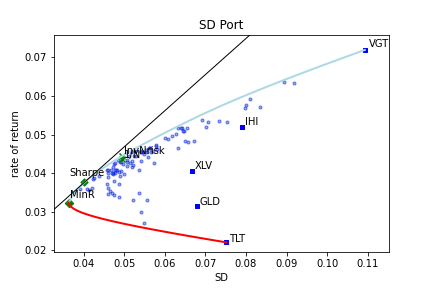
\includegraphics[width=.95\linewidth]{../figs/SDFrontier1.png}
  \caption{Rate of return vs. \SD}
  \label{SD_fig1a}
\end{subfigure}%
\begin{subfigure}{.5\textwidth}
  \centering
  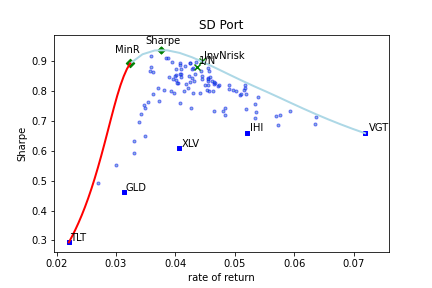
\includegraphics[width=.95\linewidth]{../figs/SDFrontier2.png}
  \caption{Sharpe vs. rate of return}
  \label{SD_fig1b}
\end{subfigure}
\caption{\SD\ frontiers.}
\label{SD_fig1}
\end{figure}

\BackToContents

\subsubsection{Backtesting Sharpe optimal portfolio}

Here is an example, using \azapy\ package, of computing a portfolio backtesting.
For this example, we have chosen a portfolio quarterly rebalanced according
to the maximization of Sharpe ratio. At each rebalancing date,
the portfolio weights
are calibrated based on 3.25 years of prior historical market data.

Other rebalancing strategies can be considered
by changing the value of {\it rtype} parameter in the call of {\it set\_model} function below.
For more details see the package documentation at \azapydoc.

\lstinputlisting[language=Python]{../PyScripts/SD_Port.py}

\begin{figure}[H]
    \centering
    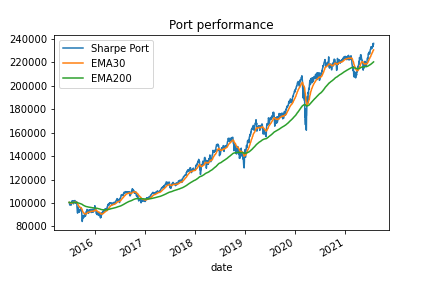
\includegraphics[width=.95\linewidth]{../figs/Port_SD_Sharpe.png}
    \caption{Backtesting of quarterly rebalanced Sharpe optimal portfolio.}
    \label{SD_Port_fig}
\end{figure}

\BackToContents

